\subsection{Disparity Testing}
After verifying that the camera interface was functional, a large portion of time was spent implementing a disparity algorithm that would allow for the extraction of 3D depth information from stereo image data. This algorithm was first implemented in \textsc{Matlab}, and was then transferred to programmable logic after the algorithm was verified working. 
\subsubsection{Image Rectification}
- ADD AN EXAMPLE OF THE MATLAB CALIBRATION STUFF (figures showing 3d anaglyph process)\par
- TALK ABOUT WHY WE DIDNT USE IN FINAL IMP


\subsubsection{\textsc{Matlab} Impelmentation}


\subsubsection{Verilog Test Bench}
The original disparity test implementation used closely follows the \textsc{Matlab} disparity algorithm shown in Appendix item \ref{disparityTestMatlab}. This algorithm is implemented using a finite state machine with five states, as shown in Figure \ref{disparityTestImp} below. In order to maintain simplicity, the test algorithm has been implemented to operate on 46x30 windowed portions of the input imagery. By default, the disparity module will remain in an idle state until an external enable signal is toggled high using a button input. This will cause the finite state machine to advance to its READ state, and image data for the left and right camera images will be read in from the stereo camera breakout board. After image data has been received, the state machine will then advance to a cyclical set of states used for iterating through each image and calculating disparity. 
\par
The disparity module will begin by isolating the template and search blocks from the right and left image data in the finite state machine's separation state. Next, the state machine will advance to its SAD state, and will calculate the sum of absolute differences between the template and search block. This value is placed in a vector that matches the length of the search range. If the vector hasn't been completely filled, indicating that there are more search blocks to compare to the template, the state machine will revert back to the separate state, isolating a new search block from the right camera image. When the SAD vector is full, the state machine will advance to its finalization state. 
\par
\begin{figure}[H]
	\centerline{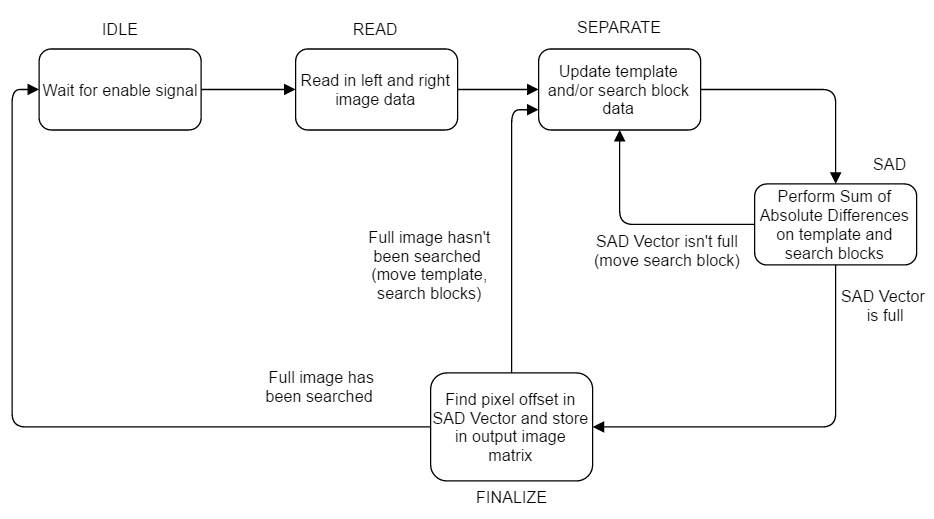
\includegraphics[width=0.75\textwidth]{looping_disparity.png}}
	\caption{Disparity Test Implementation}
	\label{disparityTestImp}
\end{figure}
\par
The finalization state is used to search through the SAD vector for the lowest value. The index of this value within the SAD vector in reference to the template block location is used to create a disparity value for the given template block location. This value is then converted to a distance using Equation \ref{disp2dist}, and is stored in the output image location. If the output image hasn't been fully populated with distance values, the state machine will then revert back to the separate state. Otherwise, the state machine will advance to its idle state, and the resulting disparity image can be read for output. 
\par
This module was initially tested using a verilog test bench, and was then tested using camera image data and a VGA display controller module, allowing for real-time verification of the algorithm's effectiveness. After testing the initial disparity algorithm, several modifications were made to increase the overall speed and efficiency of the disparity module. 
\subsubsection{Test Bench Results}
\begin{figure}[H]
	\centerline{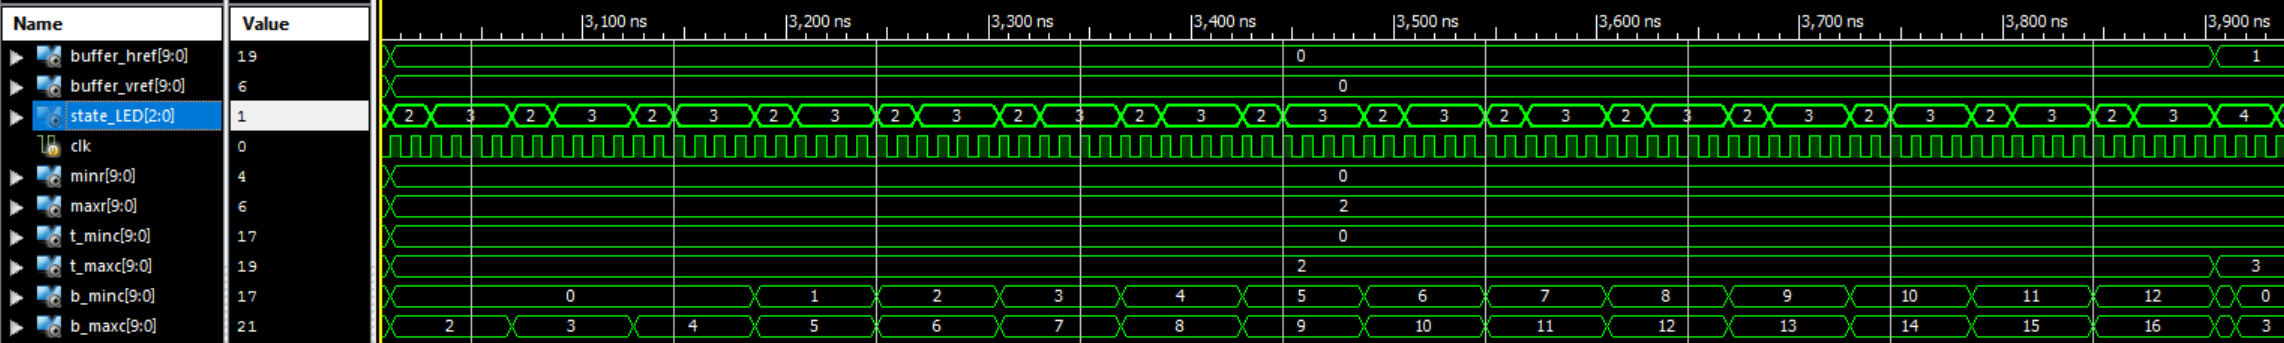
\includegraphics[width=1.25\textwidth]{disp_tb/disparity_vector.png}}
	\caption{Disparity Search Vector}
	\label{disparityVector}
\end{figure}

\begin{figure}[H]
	\centerline{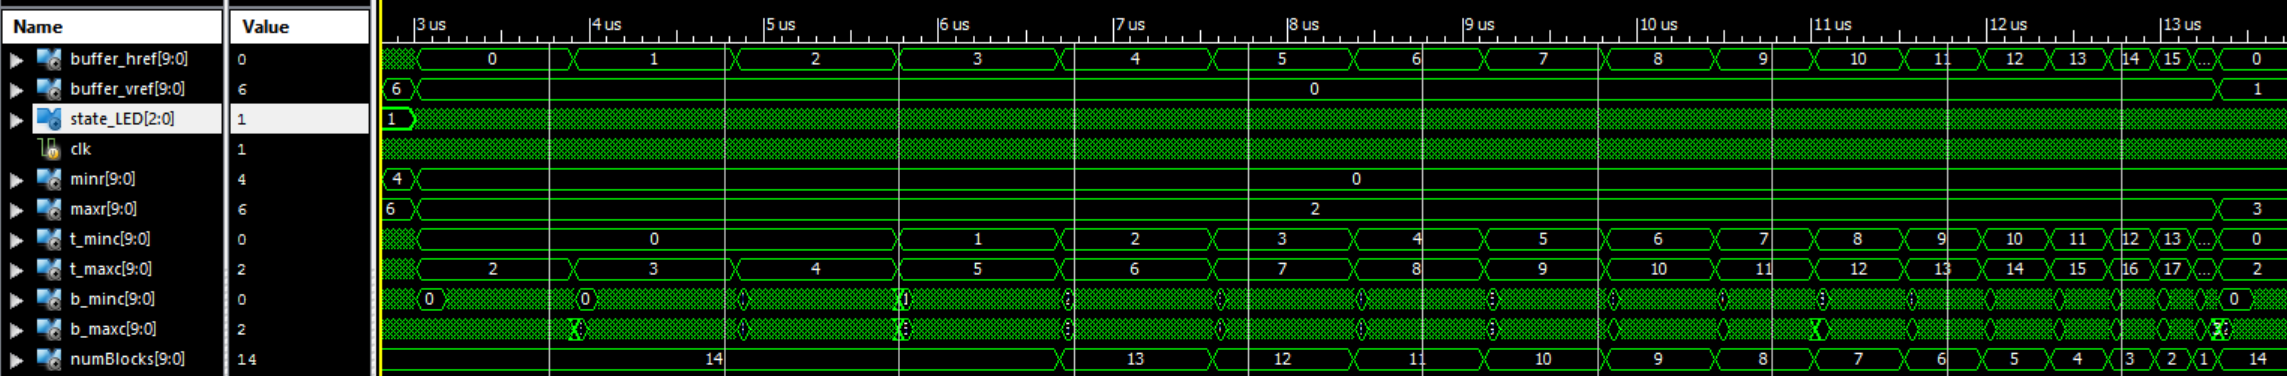
\includegraphics[width=1.25\textwidth]{disp_tb/disparity_fullPixelRow.png}}
	\caption{Horizontal Pixel Row Search}
	\label{disparityRowSearch}
\end{figure}

\begin{figure}[H]
	\centerline{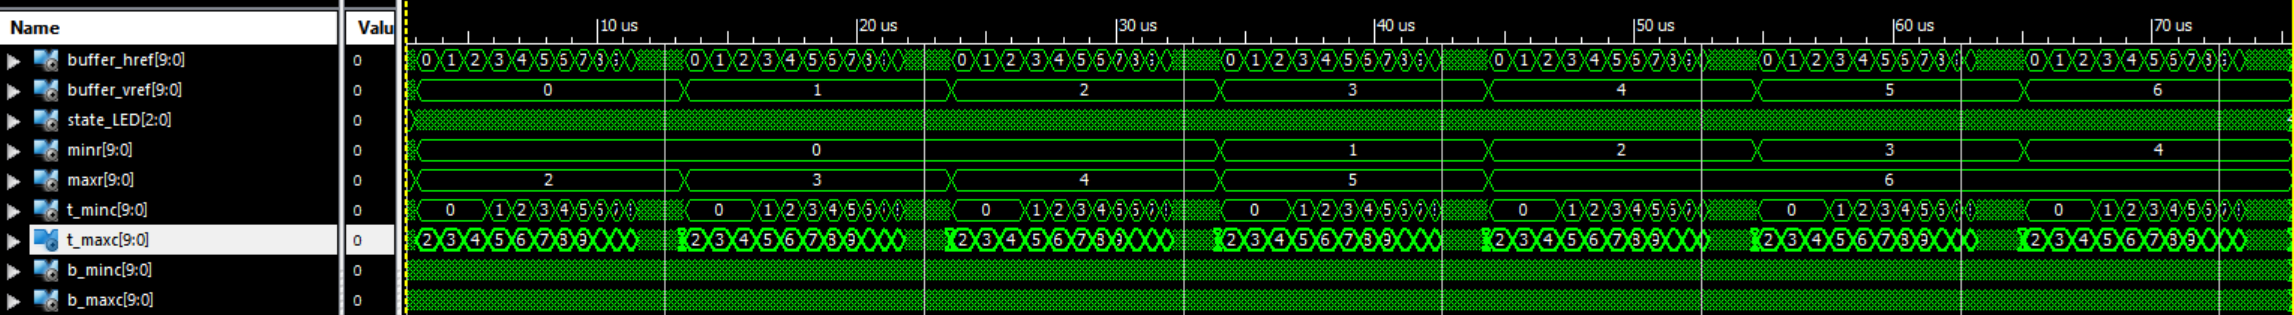
\includegraphics[width=1.25\textwidth]{disp_tb/full_disparity.png}}
	\caption{Full Image Search}
	\label{disparityFullSearch}
\end{figure}

\begin{figure}[H]
	\centerline{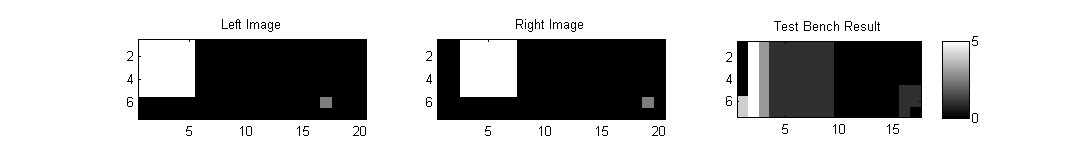
\includegraphics[width=1.0\textwidth]{disp_tb/result_gray.png}}
	\caption{Disparity Test Results}
	\label{disparityTestResults}
\end{figure}

\begin{figure}[H]
	 \begin{subfigure}[h]{1.0\textwidth}
             \centerline{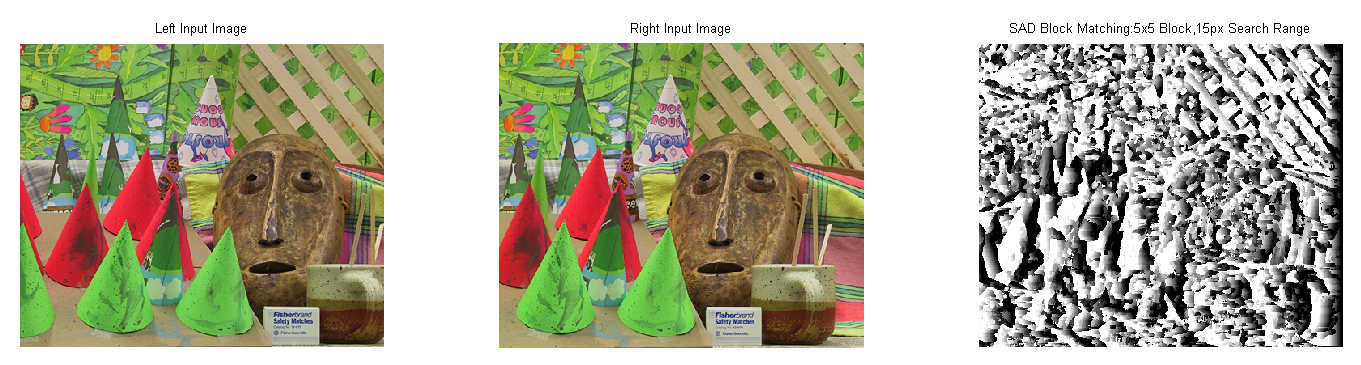
\includegraphics[width=1.2\textwidth]{disp_tb/MATLAB_cones.png}}
             \caption{\textsc{Matlab} Result}
			\label{disparityMatlabResult}
         \end{subfigure} 
         %\\
         \begin{subfigure}[h]{1.0\textwidth}
              \centerline{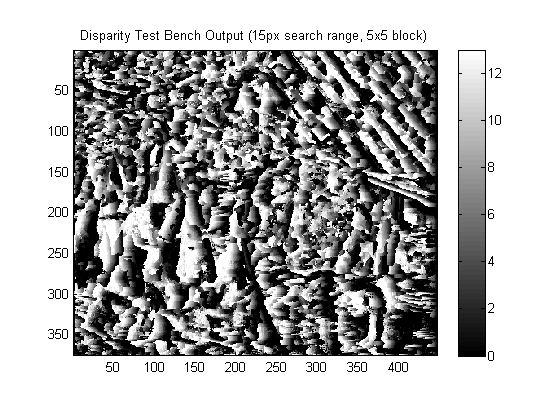
\includegraphics[width=0.66\textwidth]{disp_tb/tb_cones.png}}
             \caption{Test Bench Result}
			\label{disparityVerilogResult}
         \end{subfigure}
\label{disparityVerilogvsMatlab}
\caption{\textsc{Matlab} vs. Verilog Test Bench Results}
\end{figure}



\subsubsection{Final Implementation}
\begin{figure}[H]
	\centerline{\includegraphics[width=1.2\textwidth]{Disparity_Algorithm.png}}
	\caption{Disparity Final Implementation}
	\label{disparityTestImp}
\end{figure}
\par
GET RID OF CALIBRATION 